\documentclass[11pt,letterpaper]{article}
\usepackage[T1]{fontenc}
\usepackage[utf8]{inputenc}
\usepackage{lmodern,microtype}
\usepackage[margin=1in,headheight=14pt]{geometry}
\usepackage{amsmath,amssymb,amsthm,mathtools}
\usepackage{booktabs,longtable,array,enumitem}
\usepackage{xcolor,hyperref,fancyhdr,listings,graphicx}
\usepackage{xurl}
\definecolor{ink}{HTML}{15374A}
\definecolor{linkblue}{HTML}{176A91}
\hypersetup{colorlinks=true,linkcolor=ink,urlcolor=linkblue,citecolor=ink,
 pdftitle={Fermat's Two-Square Theorem in Intuitionistic Primitive Recursive Arithmetic},
 pdfauthor={Research report prepared for Vladimir Reshetnikov}}
\pagestyle{fancy}
\fancyhf{}
\fancyhead[L]{\small Fermat's two-square theorem in iPRA}
\fancyhead[R]{\small November 22, 2026}
\fancyfoot[C]{\thepage}
\setlength{\parskip}{4pt}
\setlength{\parindent}{15pt}
\setlist{topsep=4pt,itemsep=2pt}
\lstset{basicstyle=\ttfamily\small,columns=fullflexible,breaklines=true,
 frame=single,rulecolor=\color{black!20},xleftmargin=3pt,xrightmargin=3pt,
 keepspaces=true,showstringspaces=false}
\newtheorem{theorem}{Theorem}[section]
\newtheorem{lemma}[theorem]{Lemma}
\newtheorem{proposition}[theorem]{Proposition}
\newtheorem{corollary}[theorem]{Corollary}
\theoremstyle{definition}
\newtheorem{definition}[theorem]{Definition}
\theoremstyle{remark}
\newtheorem{remark}[theorem]{Remark}
\newcommand{\N}{\mathbb N}
\newcommand{\Z}{\mathbb Z}
\newcommand{\ipra}{\mathsf{iPRA}}
\newcommand{\pr}{\mathsf{PR}}
\newcommand{\PrimeB}{\operatorname{PrimeB}}
\newcommand{\sqroot}{\operatorname{isqrt}}
\newcommand{\remd}{\operatorname{rem}}
\newcommand{\quod}{\operatorname{quo}}
\newcommand{\abs}[1]{\lvert #1\rvert}
\newcommand{\ind}[1]{[\,#1\,]}
\newcommand{\monus}{\mathbin{\dot{-}}}
\newcommand{\Norm}{\operatorname{N}}
\newcommand{\repo}{\texttt{ProveIt}}
\newcommand{\sha}{\texttt{65b76a5b8aa87ecad4103c2d287eff5660d3c84c}}
\newcommand{\QF}{\mathsf{QF}}
\begin{document}

\begin{center}
{\color{ink}\LARGE\bfseries Fermat's Two-Square Theorem}\\[5pt]
{\Large in Intuitionistic Primitive Recursive Arithmetic}\\[10pt]
{\large Explicit witnesses, a complete finitary proof,\\
and a route to an object-level Lean derivation}\\[12pt]
Prepared for Vladimir Reshetnikov\\
November 22, 2026
\end{center}

\begin{abstract}
We prove that a prime \(p\) is a sum of two natural-number squares exactly
when \(p=2\) or \(p\equiv1\pmod4\), using intuitionistic logic and
quantifier-free induction over primitive recursive functions. The positive
direction has explicit primitive recursive witnesses. A bounded inverse
construction proves Wilson's theorem; the half-factorial gives a root of
\(-1\) modulo \(p\); a collision among \(p+1\) points in an integer square
grid produces a positive multiple of \(p\) strictly below \(2p\).
All searches have numerical bounds. We give the finite counting proof
behind the collision step, a second construction by bounded descent, a
ledger of induction invariants, executable exact-arithmetic algorithms,
and a detailed Lean implementation plan using the repository's existing
object-theory arithmetic library.
\end{abstract}

\noindent\fbox{\parbox{\dimexpr\textwidth-2\fboxsep-2\fboxrule\relax}{
\textbf{Verification boundary.}
The human-readable proof and its primitive-recursion/induction audit are
complete. The accompanying Python algorithms and certificate checks were
executed. The Lean files are an \emph{uncompiled executable specification and
conditional proof scaffold}; the required arithmetic contracts have not
been implemented, and no new closed \texttt{Prf PRAAx} derivation is claimed.
The selected upstream modules were inspected at a pinned commit but were
not recompiled in this environment.
}}

\clearpage
{\setlength{\parskip}{0pt}\small\tableofcontents}
\clearpage

\section{The exact result}

\begin{definition}[Prime predicate and represented numbers]
All unqualified variables range over \(\N\). Let
\[
 \PrimeB(n)=
 \ind{2\le n}\prod_{d<n}
 \bigl(1-\ind{2\le d}\ind{\remd(n,d)=0}\bigr).
\]
Here tests have values \(0,1\), and division by zero is totalized as described
below. Thus \(\PrimeB(n)=1\) means that \(n\ge2\) and no \(d\) with
\(2\le d<n\) divides \(n\). Write
\[
 \operatorname{Rep}(n)\;:\Longleftrightarrow\;
 \exists a\le n\;\exists b\le n\;(a^2+b^2=n).
\]
\end{definition}

\begin{theorem}[Fermat's theorem, with primitive recursive witnesses]
\label{thm:main}
There are explicitly defined total primitive recursive functions
\(A,B:\N\to\N\) such that \(\ipra\) proves
\[
 \PrimeB(p)=1\ \longrightarrow\
 \bigl(\operatorname{Rep}(p)\ \longleftrightarrow\
       (p=2\ \vee\ \remd(p,4)=1)\bigr).
\]
More strongly, \(\ipra\) proves the quantifier-free, witness-bearing implication
\[
\begin{split}
 &\PrimeB(p)=1\ \wedge\
       (p=2\ \vee\ \remd(p,4)=1)\\
 &\quad\longrightarrow\
 A(p)^2+B(p)^2=p\
 \wedge\ 1\le A(p)\le B(p)\le\sqroot(p).
\end{split}
\]
The displayed formulas stand for their universal closures.
\end{theorem}

The theorem in the question concerns odd primes. Including \(p=2\) handles
the only even prime and makes the characterization complete. The bounded
existential statement follows by introducing the terms \(A(p),B(p)\);
there is no appeal to a choice principle.

The central extraction result is slightly stronger than the prime theorem.

\begin{theorem}[A modular root gives a representation]
\label{thm:root-to-squares}
There are total primitive recursive functions \(G_1(n,t),G_2(n,t)\) for which
\(\ipra\) proves
\[
 n>0\ \wedge\ \remd(t^2+1,n)=0
 \ \longrightarrow\
 G_1(n,t)^2+G_2(n,t)^2=n.
\]
Primality is not a hypothesis here. If \(n\) is square the output is
\((0,\sqroot(n))\); otherwise a finite grid collision supplies the output.
\end{theorem}

The prime case needs Wilson's theorem only to supply the modular root.
This separates the number theory from the finite geometric argument.
The proof is an elementary reformulation, with its computational and
logical bounds made explicit; no novelty claim is made for Fermat's
theorem or the underlying classical proof ideas.

\section{Foundations: what is allowed in iPRA}
\label{sec:foundations}

\subsection{Language, axioms, and inference}

We use the usual presentation of intuitionistic primitive recursive
arithmetic: intuitionistic first-order logic with equality, symbols for
zero, successor, and each primitive recursive function, their defining
equations, the successor axioms, and the induction scheme
\[
 \bigl(C(0,\vec z)\wedge
  \forall k(C(k,\vec z)\to C(k+1,\vec z))\bigr)
 \to\forall k\,C(k,\vec z)
 \qquad(C\text{ quantifier-free}).
\]
The logical rules are the usual intuitionistic introduction and elimination
rules for \(\wedge,\vee,\to,\forall,\exists,\bot\), together with equality
substitution. In particular, arbitrary excluded middle and arbitrary
double-negation elimination are not rules.

Numerical comparisons and all finite tests in this report are decidable:
their characteristic functions are primitive recursive. A case split on
\(u=v\), \(u<v\), or a computed bit is therefore available intuitionistically.
Contradiction is used to eliminate an impossible branch of such a decision,
not to obtain an unbounded witness by classical reasoning.

This is the interface described by \repo's iPRA directory
\cite{repo-readme}. Its ordinary object-theory judgments are
\texttt{Prf PRAAx} judgments. A separate bridge transports those judgments
to the repository's alternative presentations \cite{repo-bridge}.

\subsection{Elementary total functions}

Addition, multiplication, exponentiation, truncated subtraction
\(a\monus b=\max(a-b,0)\), comparisons, and conditionals are primitive
recursive. For \(b>0\), define \(\quod(a,b)\) by the bounded largest
\(q\le a\) satisfying \(bq\le a\), and set
\[
 \remd(a,b)=a\monus b\quod(a,b).
\]
Set \(\quod(a,0)=0\) and \(\remd(a,0)=a\). A finite scan gives the quotient;
quantifier-free induction establishes, for \(b>0\),
\[
 a=b\quod(a,b)+\remd(a,b),\qquad 0\le\remd(a,b)<b.
\]
Indeed, maximality gives \(b(q+1)>a\), which bounds the remainder, and
uniqueness follows by comparing two proposed quotients. This supplies
ordinary congruence arithmetic without an external division principle.

If \(f(i,\vec z)\) is a \emph{fixed primitive recursive function}, finite
sums and products are defined by
\[
\begin{array}{ll}
 S_f(0,\vec z)=0,&S_f(k+1,\vec z)=S_f(k,\vec z)+f(k,\vec z),\\
 P_f(0,\vec z)=1,&P_f(k+1,\vec z)=P_f(k,\vec z)f(k,\vec z).
\end{array}
\]
Empty sums and products are \(0,1\). Bounded search keeps the first
successful index encountered and uses the search bound as a sentinel if
no test succeeds. Both its success property and its failure property are
proved by induction on a Boolean accumulator. Bounded minima that retain
an index are obtained by a similar scan.

These are schemas for particular fixed primitive recursive terms, or
operations on a coded finite sequence. They do \emph{not} introduce
quantification over all functions \(\N\to\N\), or a purported universal
primitive recursive evaluator.

\subsection{Bounded assertions and the induction restriction}

If \(R(i,\vec z)\) is a primitive recursive test, then
\[
 \forall i<k\,R(i,\vec z)
 \quad\text{is represented by}\quad
 \prod_{i<k}\ind{R(i,\vec z)}=1.
\]
Similarly bounded existence is represented by a nonzero sum or a
successful bounded search. Nested bounded assertions are compiled by
repeating these operations. Their intended meaning is established by
induction on the corresponding finite fold.

Consequently, a bounded assertion in an exposition is not automatically
being used as an induction formula. Before induction it is replaced by
its primitive recursive bit equation. Section~\ref{sec:audit} gives the
specific invariants needed here. There is no induction on an unbounded
existential representation statement and no use of a general least
counterexample principle.

\subsection{Signed quantities are natural-number codes}

Integers are convenient notation, not a new sort. Represent \(u-v\) by
a natural-number pair \((u,v)\). Equality, addition, negation, and
multiplication are expressed by
\[
\begin{split}
 (u,v)=(r,s)&\quad\Longleftrightarrow\quad u+s=r+v,\\
 (u,v)+(r,s)&=(u+r,v+s),\\
 -(u,v)&=(v,u),\\
 (u,v)(r,s)&=(ur+vs,us+vr).
\end{split}
\]
The absolute value is \((u\monus v)+(v\monus u)\).
For a positive modulus \(m\), the residue of \(u-v\) is
\[
 \remd\bigl(\remd(u,m)+m\monus\remd(v,m),m\bigr).
\]
The subtraction displayed here is nonnegative because
\(\remd(v,m)<m\). Thus all signed ring identities used below are identities
and comparisons between primitive recursive natural-number terms.

Pairs themselves can be encoded by
\[
 \langle u,v\rangle=(u+v)^2+u.
\]
For a code of this form, with \(s=\sqroot(\langle u,v\rangle)\), the
projections are \(u=\langle u,v\rangle\monus s^2\) and \(v=s\monus u\).
Indeed \(s=u+v\), since \(u<(u+v+1)^2-(u+v)^2\).
Nested pairs encode any fixed finite state. A length-\(k\) list with
entries less than \(D\) can instead be encoded by
\(\sum_{i<k}a_iD^i<D^k\); digit extraction and replacement are primitive
recursive. No completeness, real numbers, or set comprehension is involved.

\section{Modular inverses and Wilson's theorem}
\label{sec:wilson}

We give the finite arithmetic argument in full, rather than assume a
field or unique factorization theorem.

\begin{lemma}[A bounded inverse construction]
\label{lem:inverse}
If \(p\) is prime and \(0<a<p\), a bounded scan computes \(i<p\) with
\[
 ai\equiv1\pmod p.
\]
\end{lemma}

\begin{proof}
Among the \(p\) residues \(\remd(aj,p)\), \(0\le j<p\), choose the smallest
positive residue \(d\), retaining an index \(i\). This is a finite
algorithm: initialize the value/index pair to \((a,1)\), scan the indices,
and replace it only when a smaller positive residue is seen. The
initialization is valid because \(p\ge2\) and \(a<p\).
It gives
\[
 0<d<p,\qquad ai\equiv d\pmod p,
\]
and no positive residue in the scanned list is less than \(d\).

Divide \(p\) by \(d\):
\[
 p=qd+r,\qquad 0\le r<d.
\]
Decide whether \(r=0\). If \(r>0\), put \(j=\remd(-qi,p)\), so \(j<p\).
Then
\[
 aj\equiv-qai\equiv-qd\equiv r\pmod p.
\]
Since \(0<r<d<p\), the unique residue of \(aj\) is \(r\), contrary to
the recorded minimum. Thus \(r=0\), so \(d\mid p\). A proper positive
divisor of a prime is \(1\); hence \(d=1\), and the retained index \(i\)
is the required inverse.

There is no unbounded minimization here: the scan has \(p\) steps. Its
invariant says that the retained positive residue is attained and that
every positive residue already examined is at least as large. The latter
clause is a finite product of comparison bits.
\end{proof}

Write \(\iota(a)\) for the least \(i<p\) with \(ai\equiv1\pmod p\), using
a bounded search. Lemma~\ref{lem:inverse} shows that the sentinel is
never returned on \(0<a<p\).

\begin{lemma}[Cancellation and the inverse involution]
\label{lem:cancel}
For prime \(p\), the following assertions hold.
\begin{enumerate}
\item If \(p\nmid a\) and \(ab\equiv ac\pmod p\), then
      \(b\equiv c\pmod p\).
\item If \(p\mid ab\), then \(p\mid a\) or \(p\mid b\).
\item For \(0<a<p\), \(0<\iota(a)<p\) and \(\iota(\iota(a))=a\).
\end{enumerate}
\end{lemma}

\begin{proof}
In the first assertion, reduce \(a\) to its nonzero residue and multiply
the congruence by the inverse just constructed. For the second, decide
whether \(\remd(a,p)=0\). In that branch \(p\mid a\); in the other,
multiply \(ab\equiv0\) by the inverse to get \(b\equiv0\).
This is a constructive disjunction because the tested remainder is a number.

An inverse is nonzero, since \(0\not\equiv1\pmod p\).
If both \(u\) and \(v\) invert \(a\), multiplication by one inverse gives
\(u\equiv v\), and two residues in \(\{0,\ldots,p-1\}\) with this congruence
are equal. Since \(a\iota(a)\equiv1\) also says that \(a\) inverts
\(\iota(a)\), uniqueness proves the last assertion.
\end{proof}

\begin{lemma}[Wilson for odd primes]
\label{lem:wilson}
If \(p\) is an odd prime, then
\[
 (p-1)!\equiv-1\pmod p.
\]
\end{lemma}

\begin{proof}
The inverse map is an involution of the explicitly enumerated set
\(\{1,\ldots,p-1\}\). A fixed point \(a\) satisfies
\[
 0\equiv a^2-1=(a-1)(a+1)\pmod p.
\]
By Lemma~\ref{lem:cancel}, either \(p\mid a-1\) or \(p\mid a+1\).
The bounds \(1\le a\le p-1\) then give \(a=1\) or \(a=p-1\).
Conversely these two numbers are fixed. They are distinct because \(p\)
is odd and \(p\ge3\).

Every other entry is in a two-element pair \(\{a,\iota(a)\}\), whose
product is \(1\) modulo \(p\). Grouping these pairs therefore gives
\[
 \prod_{a=1}^{p-1}a
 \equiv 1\cdot(p-1)\cdot\prod_{\text{two-element pairs}}1
 \equiv-1\pmod p.
\]
This grouping is a finite procedure: scan the indices \(1,\ldots,p-1\),
and, at an unmarked entry, mark it and its inverse. Process a fixed entry
once and a two-element pair once. Involutivity ensures that an unmarked
entry cannot have an already marked partner. After \(p-1\) scans every
entry is marked.

For a literal induction invariant, store a bit for every marked entry and
the product, modulo \(p\), of the entries processed. That product equals
the product of the marked entries, and each nonfixed pair contributes
\(1\). The two fixed entries contribute \(1\) and \(p-1\) once each.
These are finite product equations and Boolean-fold assertions. Thus the
pairing proof uses quantifier-free induction on an explicitly bounded scan,
not a principle about arbitrary finite sets.
\end{proof}

\begin{lemma}[The half-factorial is a root of \(-1\)]
\label{lem:root}
Suppose \(\PrimeB(p)=1\) and \(p\equiv1\pmod4\). Let
\[
 H=(p-1)/2,\qquad t=\remd(H!,p).
\]
Then \(0<t<p\) and \(p\mid t^2+1\).
\end{lemma}

\begin{proof}
Write \(p=4k+1\). Primality excludes \(k=0\), so \(p\ge5\).
Then \(H=2k\) is even, and \(p-1=2H\). Reindexing the upper half of the
factorial by \(j\mapsto p-j\) gives
\[
 (p-1)!
 =\left(\prod_{j=1}^{H}j\right)
   \left(\prod_{j=1}^{H}(p-j)\right)
 \equiv (-1)^H(H!)^2
 =(H!)^2\pmod p.
\]
Wilson now gives \(t^2\equiv-1\pmod p\).
The residue definition gives \(0\le t<p\), and \(t=0\) would imply
\(p\mid1\), impossible for \(p\ge2\).

The implementation need not construct \(H!\) as a large integer. Define
\[
 F(0,p)=\remd(1,p),\qquad
 F(j+1,p)=\remd((j+1)F(j,p),p);
\]
then \(t=F(H,p)\). Induction proves \(F(j,p)\equiv j!\pmod p\).
The parity assertion and the finite reindexing above use only polynomial
identities and bounded product inductions.
\end{proof}

\section{The finite collision lemma, constructively}
\label{sec:php}

\begin{lemma}[Bounded pigeonhole principle with witnesses]
\label{lem:php}
Let \(K>0\), and let \(f(i,\vec z)\) be a fixed primitive recursive
term whose values at \(0,\ldots,K\) are less than \(K\).
Primitive recursive functions \(I,J\), obtained by bounded search, satisfy
\[
 0\le I<J\le K,\qquad f(I,\vec z)=f(J,\vec z).
\]
\end{lemma}

\begin{proof}
Search the pairs \(0\le i<j\le K\), in order of increasing \(j\), then
increasing \(i\). This has at most \(K(K+1)/2\) candidate pairs. It can
also be written as a single scan through codes \(c<(K+1)^2\), with
\[
 i=\remd(c,K+1),\qquad j=\quod(c,K+1),
\]
testing \(i<j\) and \(f(i)=f(j)\). Retain the first successful pair and
use a sentinel if every test fails.

To prove that the sentinel is impossible, define
\[
 C(n,r)=\sum_{i<n}\ind{f(i)=r},\qquad
 D(n)=\prod_{i<j<n}\bigl(1-\ind{f(i)=f(j)}\bigr).
\]
For \(n\le K+1\), each \(f(i)\) with \(i<n\) lies below \(K\), so exactly
one term in \(\sum_{r<K}\ind{f(i)=r}\) equals \(1\). Finite sum
reindexing, or induction adding one input at a time, gives
\begin{equation}
 \sum_{r<K}C(n,r)=n.
 \label{eq:mass}
\end{equation}
If \(D(n)=1\), no two of the first \(n\) values agree. We show
\begin{equation}
 D(n)=1\ \longrightarrow\ C(n,r)\le1
 \quad\text{for every numerical parameter }r.
 \label{eq:count}
\end{equation}
At \(n=0\) the count is zero. In the step to \(n+1\), \(D(n+1)=1\)
implies \(D(n)=1\) and \(f(n)\ne f(i)\) for \(i<n\).
If \(f(n)\ne r\), the count is unchanged and the induction hypothesis
applies. If \(f(n)=r\), each earlier equality bit \(\ind{f(i)=r}\) is zero,
so the old count is \(0\) and the new count is \(1\). This is a case split
on numerical equality.

If the pair scan failed at \(n=K+1\), then \(D(K+1)=1\), so
each \(C(K+1,r)\le1\). Summing these \(K\) inequalities and using
\eqref{eq:mass} yields
\[
 K+1=\sum_{r<K}C(K+1,r)\le\sum_{r<K}1=K,
\]
which is impossible. The scan's sentinel/success test is decidable.
Eliminating its impossible sentinel branch therefore proves that the
\emph{computed} indices \(I,J\) satisfy the required equalities and bounds.
\end{proof}

\begin{remark}[Exact induction formulas]
Equation~\eqref{eq:mass}, guarded by \(n\le K+1\), is quantifier-free.
For \eqref{eq:count}, use
\(D(n)=1\to C(n,r)\le1\), with \(r,K,\vec z\) free numerical parameters.
Its induction has no universal quantifier in the matrix. The finite
assertion that all earlier tests fail is represented by a Boolean
product. The final bounded sum inequality is another quantifier-free
induction. Thus \emph{pigeonhole} here is a proved arithmetic lemma with
search witnesses, not a classical cardinality axiom.
\end{remark}

\section{The square grid and the main theorem}
\label{sec:grid}

\subsection{Integer square root by primitive recursion}

Define
\[
 s(0)=0,\qquad
 s(n+1)=s(n)+\ind{(s(n)+1)^2=n+1}.
\]
Quantifier-free induction proves
\begin{equation}
 s(n)^2\le n<(s(n)+1)^2.
 \label{eq:sqrt}
\end{equation}
For the induction step, let \(r=s(n)\). If \((r+1)^2=n+1\), the
recurrence advances to \(r+1\), and \((r+1)^2<(r+2)^2\).
Otherwise \(n+1<(r+1)^2\), since \(n<(r+1)^2\) and the quantities are
integers; the recurrence stays at \(r\).
In either branch the lower bound is immediate. Set \(\sqroot(n)=s(n)\).
The notation \(\lfloor\sqrt n\rfloor\) below means this function; no
real square-root operation is used.

\subsection{Root-to-squares extraction}

\begin{proof}[Proof of Theorem~\ref{thm:root-to-squares}]
Let \(n>0\), \(n\mid t^2+1\), \(h=\sqroot(n)\), and \(B=h+1\).
First decide whether \(h^2=n\). If so, return \((0,h)\).
Otherwise \eqref{eq:sqrt} gives
\[
 h^2<n<B^2.
\]
For each index \(0\le i\le n\), define
\[
 u_i=\remd(i,B),\qquad v_i=\quod(i,B).
\]
Division gives \(i=u_i+Bv_i\) and \(0\le u_i<B\).
Since \(i\le n<B^2\), necessarily \(v_i<B\): if \(v_i\ge B\),
then \(i\ge Bv_i\ge B^2\), a contradiction. Hence
\[
 0\le u_i\le h,\qquad 0\le v_i\le h.
\]
Distinct indices give distinct ordered pairs, because the equation
\(i=u_i+Bv_i\) reconstructs the index.

Label these \(n+1\) points by the \(n\) possible residues
\[
 f(i)=\remd(u_i+t v_i,n).
\]
The finite collision lemma computes \(i<j\le n\) with \(f(i)=f(j)\).
Put
\[
 x=u_j-u_i,\qquad y=v_j-v_i.
\]
At least one difference is nonzero, since the two points are distinct.
The collision gives \(x+ty\equiv0\pmod n\), and hence
\[
 x^2+y^2\equiv (t^2+1)y^2\equiv0\pmod n.
\]
Equivalently, the polynomial identity
\begin{equation}
 x^2+y^2=(x+ty)(x-ty)+(t^2+1)y^2
 \label{eq:divisible}
\end{equation}
expresses the norm as a sum of two multiples of \(n\).
Both \(\abs{x}\) and \(\abs{y}\) are at most \(h\), so
\begin{equation}
 0<x^2+y^2\le2h^2<2n.
 \label{eq:shortnorm}
\end{equation}
Write \(x^2+y^2=nq\), using exact quotient extraction.
Positivity and \(n>0\) give \(q\ge1\), while \(nq<2n\) gives \(q<2\).
Thus \(q=1\) and
\[
 x^2+y^2=n.
\]
Return the sorted pair
\[
 G_1(n,t)=\min(\abs{x},\abs{y}),\qquad
 G_2(n,t)=\max(\abs{x},\abs{y}).
\]
All functions in this construction are totalized on inputs not satisfying
the hypotheses by the same finite search with a sentinel and a fixed
fallback pair. The theorem only asserts correctness under its explicit
premise. Every search and iteration bound has already been specified.
\end{proof}

\subsection{Positive direction for primes}

For \(p=2\), set \(A(p)=B(p)=1\).
For every other input define
\[
 A(p)=G_1(p,F((p\monus1)/2,p)),\qquad
 B(p)=G_2(p,F((p\monus1)/2,p)).
\]
These are total primitive recursive functions. If \(p\) is prime and
\(p\equiv1\pmod4\), Lemma~\ref{lem:root} supplies the hypothesis of
Theorem~\ref{thm:root-to-squares}, which gives \(A(p)^2+B(p)^2=p\).

A prime is not a square. Indeed, if \(p=h^2\), then \(h=0\) gives \(p=0\)
and \(h=1\) gives \(p=1\); if \(h\ge2\), then \(h\mid p\) and
\(2\le h<h^2=p\), contrary to primality. Thus the grid branch applies
to every odd target prime. Its output is bounded by \(h=\sqroot(p)\).
Neither output can be zero, since that would again make \(p\) a square.
Sorting gives \(1\le A(p)\le B(p)\le h\).

\subsection{Converse and the even prime}

For any \(z\in\N\), divide by \(2\): \(z=2q+r\), \(r=0\) or \(1\).
Expanding the square shows
\[
 z^2\equiv r^2\in\{0,1\}\pmod4.
\]
Consequently a sum of two squares is congruent to \(0,1,\) or \(2\)
modulo \(4\), and cannot be congruent to \(3\).

If a prime \(p\) is even, then \(2\mid p\). Deciding \(p=2\) versus
\(p>2\), the second branch would make \(2\) a forbidden proper divisor.
Hence the only even prime is \(2\). An odd prime has residue \(1\)
or \(3\) modulo \(4\), by division and the four residue cases.
If it is represented by two squares, residue \(3\) is impossible;
therefore its residue is \(1\). This proves the reverse implication
of Theorem~\ref{thm:main}.

\subsection{A worked example}

Take \(p=1009\). The modular factorial computation gives
\[
 t=504!\bmod1009=540,\qquad 540^2+1=289\cdot1009.
\]
Here \(h=31\), \(B=32\). The first collision in the prescribed order is
\[
 i=28,\quad (u_i,v_i)=(28,0),\qquad
 j=480,\quad (u_j,v_j)=(0,15),
\]
because \(540\cdot15\equiv28\pmod{1009}\).
The differences are \(x=-28,y=15\), so the output is
\[
 \boxed{1009=15^2+28^2}.
\]
The output is certified by exact integer arithmetic; the general proof
of success is the preceding argument.

\begin{figure}[htbp]
\centering
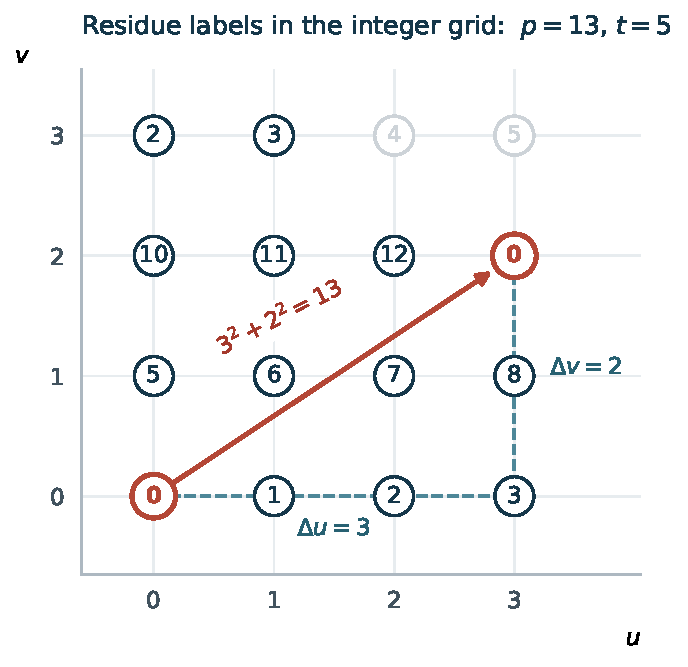
\includegraphics[width=.73\textwidth]{figures/grid_p13.pdf}
\caption{The first 14 points of the \(4\) by \(4\) grid for \(p=13\), \(t=5\).
Each label is \(u+5v\) modulo \(13\). The highlighted equal labels at
\((0,0)\) and \((3,2)\) give \(13=3^2+2^2\); the two pale points are
outside the indexed prefix.}
\label{fig:grid}
\end{figure}

\section{An independent construction by bounded descent}
\label{sec:descent}

The grid proof already establishes the theorem. This second construction
provides an independent arithmetic route to witnesses and a useful
comparison with the repository's clocked-descent infrastructure.

\subsection{Initial state}

Let \(p\) be prime, \(p\equiv1\pmod4\), and choose \(t\) as above.
Since \(0<t<p\),
\[
 0<t^2+1\le(p-1)^2+1<p^2.
\]
Set \(m_0=(t^2+1)/p\), \(a_0=t\), \(b_0=1\). Then
\[
 1\le m_0<p,\qquad a_0^2+b_0^2=m_0p.
\]
We maintain the invariant
\begin{equation}
 1\le m<p,\qquad a^2+b^2=mp,
 \label{eq:descentinv}
\end{equation}
where \(a,b\) are signed integers represented by natural-number codes.

\subsection{One descent step}

If \(m=1\), keep the state unchanged. If \(m>1\), choose centered
residues \(r,s\) of \(a,b\) modulo \(m\). Explicitly, for a residue
\(e\in\{0,\ldots,m-1\}\), use \(e\) if \(2e\le m\), and \(e-m\) otherwise.
Thus
\[
 r\equiv a,\quad s\equiv b\pmod m,\qquad
 2\abs r\le m,\quad 2\abs s\le m.
\]
Since \(m\mid a^2+b^2\), it also divides \(r^2+s^2\). Define
\[
 m'=\frac{r^2+s^2}{m}.
\]
We first prove \(m'>0\). If \(r=s=0\), then \(m\mid a\) and \(m\mid b\);
write \(a=mu,b=mv\). From \(a^2+b^2=mp\), cancellation of \(m>0\) gives
\[
 p=m(u^2+v^2).
\]
Thus \(m\mid p\), contrary to \(1<m<p\) and primality. At least one of
\(r,s\) is nonzero, so \(r^2+s^2>0\) and \(m'>0\).

The centered bounds give
\[
 4(r^2+s^2)\le2m^2.
\]
Substituting \(r^2+s^2=mm'\) and cancelling positive factors gives
\begin{equation}
 2m'\le m,\qquad 1\le m'<m.
 \label{eq:half}
\end{equation}
This includes the boundary case \(m=2\), where necessarily \(m'=1\).

The quantities \(ar+bs\) and \(br-as\) are divisible by \(m\), because
\[
 ar+bs\equiv a^2+b^2\equiv0,\qquad
 br-as\equiv ba-ab=0\pmod m.
\]
Define the exact signed quotients
\[
 a'=\frac{ar+bs}{m},\qquad b'=\frac{br-as}{m}.
\]
The identity
\[
 (ar+bs)^2+(br-as)^2=(a^2+b^2)(r^2+s^2)
\]
now yields
\[
 m^2(a'^2+b'^2)=(mp)(mm')=m^2pm'.
\]
Cancelling \(m^2>0\) proves \(a'^2+b'^2=pm'\).
Together with \eqref{eq:half}, this preserves \eqref{eq:descentinv}.
The quotients are computed by totalized integer division; exactness is
proved from the invariant, rather than built in as an unbounded search.

\subsection{Fixed fuel, rather than unbounded descent}

Let \(D_p\) be this total guarded step, and define
\[
 S(0)=S_0,\qquad S(k+1)=D_p(S(k))
\]
by primitive recursion, keeping a state of multiplier \(1\) fixed.
Write \(m_k\) for its multiplier.
Quantifier-free induction proves both \eqref{eq:descentinv} and
\begin{equation}
 m_k=1\quad\vee\quad m_k+k\le m_0.
 \label{eq:clock}
\end{equation}
At \(k=0\), the second disjunct holds. For the step, a multiplier \(1\)
stays \(1\); otherwise \(m_{k+1}+1\le m_k\), and the second disjunct
propagates unless the first has already become true.

At \(k=p\), the second disjunct would imply
\(m_p+p\le m_0<p\), impossible. Hence \(m_p=1\), and the absolute values
of the final signed coordinates are a representation of \(p\).
The implementation therefore runs exactly \(p\) iterations; it does not
use a general theorem asserting termination of arbitrary decreasing
processes. The stronger inequality \(2m'\le m\) explains why far fewer
active steps occur in examples, but the proof needs only the simple
primitive recursive fuel bound.

\section{Why the proof stays inside iPRA}
\label{sec:audit}

\subsection{Induction ledger}

The following ledger identifies the actual induction objects. A bounded
universal clause in the description is represented by a primitive
recursive product of bits before applying induction.

\begin{longtable}{@{}>{\raggedright\arraybackslash}p{0.19\textwidth}>{\raggedright\arraybackslash}p{0.47\textwidth}>{\raggedright\arraybackslash}p{0.27\textwidth}@{}}
\toprule
Construction & Quantifier-free invariant or equation & Bound / purpose\\
\midrule
\endfirsthead
\toprule Construction & Quantifier-free invariant or equation & Bound / purpose\\
\midrule
\endhead
Bounded search &
The retained index is the first success in the scanned prefix, or the
sentinel and all scanned test bits are zero. &
The supplied bound is a natural-number term.\\
\addlinespace
Division &
\(a=bq+r\), \(r<b\), after the quotient/remainder scan. &
At most \(a+1\) quotient candidates for \(b>0\).\\
\addlinespace
Integer square root &
\(s(n)^2\le n<(s(n)+1)^2\). &
\(n\) applications of its recurrence.\\
\addlinespace
Minimum positive residue &
The stored residue is positive, attained at a stored index, and no
positive examined residue is smaller. &
\(p\) residue candidates; the initial candidate is \(a\).\\
\addlinespace
Wilson pairing &
The marked entries form inverse pairs and fixed points; the stored
product is their product modulo \(p\). &
\(p-1\) scans; a finite bitmask.\\
\addlinespace
Modular factorial &
\(F(j,p)\equiv j!\pmod p\), \(F(j,p)<p\) for \(p>0\). &
\((p-1)/2\) modular multiplications.\\
\addlinespace
Counting inputs &
\(n\le K+1\to\sum_{r<K}C(n,r)=n\). &
Induction on prefix length \(n\).\\
\addlinespace
No repeated value &
\(D(n)=1\to C(n,r)\le1\), with \(r\) a free number parameter. &
Induction on prefix length \(n\).\\
\addlinespace
Summing inequalities &
The sum of the first \(v\) counts is at most \(v\) when each corresponding
count is at most \(1\). &
At most \(K\) additions.\\
\addlinespace
Optional descent &
\(1\le m_k<p\), \(a_k^2+b_k^2=pm_k\), and
\(m_k=1\vee m_k+k\le m_0\). &
Exactly \(p\) state transitions.\\
\bottomrule
\end{longtable}

For example, the minimum-residue invariant has the form
\[
 0<d_k<p\ \wedge\ \remd(ai_k,p)=d_k\ \wedge\
 \prod_{j<k}
 \ind{\remd(aj,p)=0\ \vee\ d_k\le\remd(aj,p)}=1,
\]
with a harmless extra assertion for the initialized candidate.
Every displayed component is quantifier-free in the PR-enriched language.
The relation between the product and its bounded reading is proved by
the same elementary fold induction used for bounded search.

If primality is written in its usual quantified form, it can stay as a
fixed assumption in the induction context. Alternatively use
\(\PrimeB(p)=1\), which is literally quantifier-free.
An induction hypothesis must not silently contain the repository's
quantified \texttt{prime} formula as if it were QF.

\subsection{No hidden infinitary step}

The proof never takes a minimum over an unbounded set, chooses elements
from an arbitrary family of nonempty sets, uses real analysis or Gaussian
unique factorization, or appeals to induction for a formula containing an
unbounded existential. Signed expressions are encoded natural-number
calculations. The root and collision are actual computed terms.

The only contradictions used to prove existence are contradictions in
decidable finite branches: a zero remainder versus a positive one, or a
bounded search sentinel versus success. The witness is already part of
the finite computation. This is intuitionistically valid.

\subsection{Size and termination bounds}

The modular factorial has fewer than \(p\) steps; integer square root has
\(p\) steps; the direct collision scan has at most \((p+1)^2\) tests.
Thus the displayed witness construction has a simple primitive recursive
bound, polynomial in the \emph{numerical value} \(p\) when arithmetic
operations are counted as single operations. This is not a claim of
polynomial running time in the binary length \(\log p\).

An efficient finite-table realization of the collision scan uses \(p\)
entries and \(p+1\) iterations, recording the first index with each label.
Each entry lies in \(0,\ldots,p+1\); as one natural-number code, the table
is less than \((p+2)^p\). The table is still a legitimate PR object.
The shipped Python program compares this table implementation against
the direct bounded pair search on finite test families.

\section{Lean formalization: definitions, dependencies, and remaining work}
\label{sec:lean}

\subsection{Three distinct layers}

It is useful to separate three statements:
\begin{enumerate}
\item the arithmetic program computes particular correct examples;
\item Lean proves a theorem about ordinary \texttt{Nat} and that program;
\item Lean constructs an object-theory derivation
      \texttt{Prf PRAAx [] phi} for the corresponding first-order sentence.
\end{enumerate}
Only the third is a kernel-checked formal proof that the sentence is
derivable in the specified iPRA calculus. This package supplies executed
evidence for the first, a human proof of the theorem with its iPRA audit,
and an uncompiled specification and explicit contracts for the second.
It gives the dependency and construction plan for the third; it does not
claim to have completed that object-level derivation.

\subsection{Available definitions in the supplied Lean project}

The standalone project targets Lean \texttt{v4.32.0}, matching the
inspected repository toolchain. Its principal computational definitions
are natural-number recursions: numerical primality testing, modular
factorial, integer square root, bounded first-hit search, grid coordinate
and label computation, collision decoding, absolute difference, and the
representation witness.

The Lean outline enumerates pair codes with
\(i=\quod(c,p+1)\), \(j=\remd(c,p+1)\), and leaves the two output
coordinates unsorted. The report and Python reference order the search
by \(j\), then \(i\), and sort the output. These constructions satisfy
the same representation specification but need not return identical
ordered pairs. A final \(\min/\max\) wrapper gives the sorted bounds.
The Lean contracts target the prime theorem; the Python reference also
implements the square-modulus branch of the stronger root-to-squares lemma.

The \texttt{ArithmeticContracts} structure records the mathematical lemmas
needed to connect those definitions. A conditional theorem assembles the
prime result from a value of that structure. No such value is supplied.
Thus the conditional assembly neither assumes the contracts as global
axioms nor pretends that they have been proved. The project contains no
\texttt{sorry} or newly declared \texttt{axiom}. Absence of those tokens
does not by itself certify the theorem; the contracts and the uncompiled
status remain explicit.

The accompanying Lean README and roadmap give the exact declaration
names and completion order. A small result checker verifies the equation
for a supplied pair, separately from proving that the search always
succeeds. An optional Mathlib comparison, described in the roadmap, is a
statement-level check and cannot replace the iPRA derivation.
Mathlib already contains \texttt{Nat.Prime.sq\_add\_sq}, proved through
Gaussian-integer infrastructure \cite{mathlib}; this report uses the
finite arithmetic route to control the induction strength.

\subsection{Pinned repository reuse}

The repository was inspected at commit
\[
 \texttt{65b76a5b8aa87ecad4103c2d287eff5660d3c84c}.
\]
The source README describes its \texttt{IPRADerivations} library as
kernel checked. We inspected declarations and proof bodies; we did not
independently rerun that build. The relevant module names are relative
to \texttt{IPRADerivations}.

\begin{longtable}{@{}>{\raggedright\arraybackslash}p{0.32\textwidth}>{\raggedright\arraybackslash}p{0.30\textwidth}>{\raggedright\arraybackslash}p{0.31\textwidth}@{}}
\toprule
Module & Existing declarations & Role here\\
\midrule
\endfirsthead
\toprule Module & Existing declarations & Role here\\
\midrule
\endhead
\texttt{Core.Pairing} &
\texttt{isqrtF}, \texttt{isqrt}, \texttt{isqrt\_le},
\texttt{lt\_isqrt\_succ\_sq} &
The exact PR square-root recurrence and its two inequalities.\\
\addlinespace
\texttt{Core.Pigeonhole} &
\texttt{phpI}, \texttt{phpJ}, \texttt{pigeonhole} &
Explicit collision terms and an object-theory derivation of their specification.\\
\addlinespace
\texttt{Core.Division} &
\texttt{remF}, \texttt{quoF}, \texttt{div\_mod},
\texttt{div\_mod\_unique} &
Remainder bounds, coordinate reconstruction, exact quotient extraction.\\
\addlinespace
\texttt{Core.Search} &
\texttt{Search.mu}, \texttt{search\_spec},
\texttt{search\_found} &
Bounded inverse and collision searches.\\
\addlinespace
\texttt{Core.EuclidLemma} &
\texttt{euclid\_lemma\_at}, \texttt{gcd\_prime},
\texttt{bezout\_at} &
An existing alternative to the bounded minimum proof of inverses.\\
\addlinespace
\texttt{Core.Permutation} and \texttt{Core.ProdLemmas} &
\texttt{Permutation.prod\_perm},
\texttt{prod\_congr\_bounded} &
Finite product rearrangement for Wilson and the half-factorial.\\
\addlinespace
\texttt{Foundations.}\newline\texttt{BoundedFormulas} &
\texttt{bf\_reflect}, \texttt{bf\_choice}, \texttt{bf\_least} &
Compile bounded assertions to PR characteristic terms.\\
\addlinespace
\texttt{Core.Quotient} and \texttt{Core.IntCertificates} &
\texttt{Q.exact}, \texttt{Q.sound}, \texttt{nn\_zsq} &
Object-theory polynomial identities and signed-square inequalities.\\
\addlinespace
\texttt{Core.ClockedDescent} &
\texttt{iterF}, \texttt{orb}, \texttt{clocked\_at} &
Optional descent alternative; use a guarded termination invariant as above.\\
\bottomrule
\end{longtable}

In particular, the repository's pigeonhole theorem has the actual
object-theory shape
\begin{lstlisting}
theorem pigeonhole {K x : PTm n}
    (hr : Gamma |- [PRAAx] Permutation.rangeAll S K x) :
    Gamma |- [PRAAx]
      lt (phpI S K x) (phpJ S K x) /\
      (le (phpJ S K x) K /\
       inst2 S (phpI S K x) x =
       inst2 S (phpJ S K x) x)
\end{lstlisting}
Here the listing uses ASCII stand-ins for the repository's formula and
derivability notation; the exact Unicode declaration is recorded in the
source-context file. Its \texttt{rangeAll} premise concerns all numerical
inputs. The grid label's final remainder modulo \(p>0\) gives the required
global range bound, even though coordinate bounds are only used for
indices at most \(p\).

\subsection{A concrete implementation sequence}

\begin{enumerate}
\item \textbf{Encode the numerical terms.}
Use \texttt{rec1}/simultaneous recursion for \(F\), reuse
\texttt{isqrtF}, and define \(B=h+1\), coordinates, and
the label term \(S(i,p)=\remd(u_i+t(p)v_i,p)\).
Use the existing \texttt{phpI/phpJ} terms instead of creating a new
pigeonhole proof. The executable search and these library terms may
select witnesses differently; both are primitive recursive and both
satisfy the same specification.

\item \textbf{Supply the Wilson endpoint.}
Either formalize Lemma~\ref{lem:inverse}'s bounded-minimum scan, or use
the checked B\'ezout and Euclid lemmas to produce inverses.
Prove inverse uniqueness, involutivity, fixed-point classification,
and the finite product identity by object derivations.
Then prove the half-factorial congruence. These are the main new
number-theoretic obligations.

\item \textbf{Instantiate pigeonhole.}
Derive the label range using \texttt{div\_mod}. Apply the
\texttt{pigeonhole} endpoint to obtain \(i<j\le p\) and label equality.
Unpack the square-root bounds and derive the coordinate bounds.

\item \textbf{Compile the short-norm calculation.}
Use natural difference codes for \(x,y\), the ring-identity compiler for
\eqref{eq:divisible}, and order lemmas for
\(0<x^2+y^2<2p\).
Derive positivity from coordinate reconstruction and \(i\ne j\).
Extract the quotient and prove it equals \(1\).

\item \textbf{Finish the prime theorem.}
Rule out a prime square, handle \(p=2\), and prove the mod-\(4\)
converse by four residue cases. Introduce the explicit output terms
as existential witnesses if the traditional statement is desired.

\item \textbf{Close and audit the object proof.}
Universally close the free numerical parameters, yielding an empty-context,
scope-zero \texttt{Prf PRAAx} proof. Inspect its dependency graph for the
permitted axioms. If the alternate Foundation presentation is wanted,
apply the repository's checked \texttt{IPRABridge.conciseToStandard}.
\end{enumerate}

The intended witness endpoint, in mathematical syntax, is
\[
 []\vdash_{\mathrm{PRAAx}}\forall p\,
 \bigl(\PrimeB(p)=1\wedge(p=2\vee\remd(p,4)=1)
 \to A(p)^2+B(p)^2=p\bigr).
\]
The required PR symbols, bounds, and local proof obligations have all
been specified; the remaining work is their Lean construction and checking.

\section{Executed validation and reproducibility}
\label{sec:validation}

\subsection{Validation results}

The Python programs use only the standard library and exact integers.
The recorded run used Python \texttt{3.12.14} and the bound \(20{,}000\).
The following checks passed:

\begin{center}
\begin{tabular}{@{}p{0.73\textwidth}r@{}}
\toprule
Check & Cases\\
\midrule
All primes through \(20{,}000\), compared with an independently enumerated
table of sums of two squares & \(2262\)\\
Odd primes \(p\equiv1\pmod4\), grid certificates verified & \(1125\)\\
The same primes, independent descent certificates verified & \(1125\)\\
Primality and integer-square-root comparisons, \(0\le n\le1000\) & \(1001\)\\
Table collision versus direct bounded pair scan, every residue for
\(1\le n\le80\) & \(3240\)\\
All roots of \(-1\) for every modulus \(1\le n\le200\) & \(98\)\\
All valid signed descent states \(\abs a,\abs b<p\), \(1\le m<p\),
for primes \(p\le101\) & \(3772\)\\
\bottomrule
\end{tabular}
\end{center}

The modular factorial was also compared with the ordinary exact factorial
for primes at most \(500\). A deliberately changed output coordinate was
rejected by the independent grid certificate checker for every target
prime tested. The longest active descent in the main run had six steps,
first attained at \(p=19073\); the program still used the fixed \(p\)-step
fuel bound.

The finite tests support the implementations and catch boundary mistakes;
they do not prove the universal theorem. That proof is
Sections~\ref{sec:wilson}--\ref{sec:audit}.

\subsection{Selected computed witnesses}

\begin{center}
\begin{tabular}{@{}rrrrrr@{}}
\toprule
\(p\) & \(t\) & \(h\) & \(i,j\) & \(A(p),B(p)\) & Descent steps\\
\midrule
5 & 2 & 2 & \(2,3\) & \(1,2\) & 0\\
13 & 5 & 3 & \(0,11\) & \(2,3\) & 1\\
17 & 13 & 4 & \(0,9\) & \(1,4\) & 1\\
41 & 9 & 6 & \(0,33\) & \(4,5\) & 1\\
97 & 22 & 9 & \(0,49\) & \(4,9\) & 1\\
1009 & 540 & 31 & \(28,480\) & \(15,28\) & 2\\
10009 & 6706 & 100 & \(100,303\) & \(3,100\) & 2\\
19997 & 17695 & 141 & \(139,3692\) & \(26,139\) & 4\\
\bottomrule
\end{tabular}
\end{center}

\subsection{Commands and artifact status}

From the package root:
\begin{lstlisting}
python3 python/two_squares.py 1009
python3 python/validate.py --limit 20000
pdflatex -interaction=nonstopmode -halt-on-error fermat_two_squares_ipra.tex
pdflatex -interaction=nonstopmode -halt-on-error fermat_two_squares_ipra.tex
\end{lstlisting}
For the uncompiled Lean project, install the pinned toolchain, enter
\texttt{lean/}, and run \texttt{lake build}. Successful compilation of
the scaffold would still leave the arithmetic contracts and object
derivation to be implemented.

The archive contains the report source and compiled PDF; Python
constructors and certificate verifiers; recorded validation and examples;
the Lean executable specification, contract interface, and roadmap; and
repository provenance. See \texttt{README.md} for the file map and
\texttt{validation/validation.json} for machine-readable run results.

\section{Scope of the conclusion}

Fermat's prime two-square theorem admits a direct proof with explicit
primitive recursive witnesses and quantifier-free induction.
The finite grid is especially useful for this goal: after the modular
root is obtained, the whole existence proof is a bounded collision
calculation followed by the inequality \(0<N<2p\).
The stronger root-to-squares lemma and the independent bounded descent
are established in the same constructive setting.

The mathematical result and the formalization plan have different
completion statuses. The former is proved here; the new Lean object
derivation remains to be implemented. The repository already supplies
several of the required object-level arithmetic components, which makes
the remaining route concrete without confusing it with a completed
kernel check.

\begin{thebibliography}{99}
\small
\raggedright
\bibitem{target}
Fermat's theorem on sums of two squares, the user-specified theorem
statement. \url{https://en.wikipedia.org/wiki/Fermat%27s_theorem_on_sums_of_two_squares}.
Accessed November 22, 2026. Used to identify the requested theorem;
the proof in this report is self-contained.

\bibitem{repo-readme}
Vladimir Reshetnikov, \emph{ProveIt: Primitive recursive arithmetic},
README at commit \sha.
\url{https://github.com/VladimirReshetnikov/ProveIt/blob/65b76a5b8aa87ecad4103c2d287eff5660d3c84c/Logic/PrimitiveRecursiveArithmetic/README.md}.

\bibitem{repo-bridge}
\emph{ProveIt: iPRA Bridge}, README at the same commit.
\url{https://github.com/VladimirReshetnikov/ProveIt/blob/65b76a5b8aa87ecad4103c2d287eff5660d3c84c/Logic/PrimitiveRecursiveArithmetic/Bridge/README.md}.

\bibitem{repo-pairing}
\emph{ProveIt: Core.Pairing}, integer square root, pairing, and
simultaneous recursion, at the same commit.
\url{https://github.com/VladimirReshetnikov/ProveIt/blob/65b76a5b8aa87ecad4103c2d287eff5660d3c84c/Logic/PrimitiveRecursiveArithmetic/Derivations/Lean/IPRADerivations/Core/Pairing.lean}.

\bibitem{repo-php}
\emph{ProveIt: Core.Pigeonhole}, explicit PR collision witnesses, at the
same commit.
\url{https://github.com/VladimirReshetnikov/ProveIt/blob/65b76a5b8aa87ecad4103c2d287eff5660d3c84c/Logic/PrimitiveRecursiveArithmetic/Derivations/Lean/IPRADerivations/Core/Pigeonhole.lean}.

\bibitem{repo-bounded}
\emph{ProveIt: Foundations.BoundedFormulas}, bounded formula
reflection and witness extraction, at the same commit.
\url{https://github.com/VladimirReshetnikov/ProveIt/blob/65b76a5b8aa87ecad4103c2d287eff5660d3c84c/Logic/PrimitiveRecursiveArithmetic/Derivations/Lean/IPRADerivations/Foundations/BoundedFormulas.lean}.

\bibitem{repo-euclid}
\emph{ProveIt: Core.EuclidLemma}, prime cancellation and B\'ezout
interfaces, at the same commit.
\url{https://github.com/VladimirReshetnikov/ProveIt/blob/65b76a5b8aa87ecad4103c2d287eff5660d3c84c/Logic/PrimitiveRecursiveArithmetic/Derivations/Lean/IPRADerivations/Core/EuclidLemma.lean}.

\bibitem{mathlib}
Chris Hughes and Michael Stoll, \emph{Mathlib.NumberTheory.SumTwoSquares}.
The ordinary Lean theorem \texttt{Nat.Prime.sq\_add\_sq} is a comparison
endpoint, not an iPRA dependency of this proof.
\url{https://github.com/leanprover-community/mathlib4/blob/master/Mathlib/NumberTheory/SumTwoSquares.lean}.
Inspected November 22, 2026; this moving URL is not a build pin.
\end{thebibliography}

\end{document}
